\section{A Brief Introduction to Quantum Computing}
\label{sec:qc}

\subsection{Meet the Qubit}
\label{sec:qubit}

A quantum bit, know as a qubit, is the basic unit of quantum information. The 
principle behind \gls{qc} is to take advantage of the properties of quantum 
mechanics for computations and information processing such as superposition and 
entanglement. A classic bit can only have a value of 0 or 1, a qubit can be in a
superposition of 0 and 1. The Bloch sphere~\cite{Bloch} is a geometrical 
representation of the pure state space of a qubit as is shown in Figure~\ref{fig:bloch}. 
This is a useful representation of a qubit where one can think of the sate of a 
qubit as a vector inside a 3-D sphere. The north and south poles of the Bloch 
sphere are typically chosen to correspond to the standard basis vectors $\vert 0 \rangle$
and $\vert 1 \rangle$ respectively.

\begin{figure}[!htbp]
\centering
	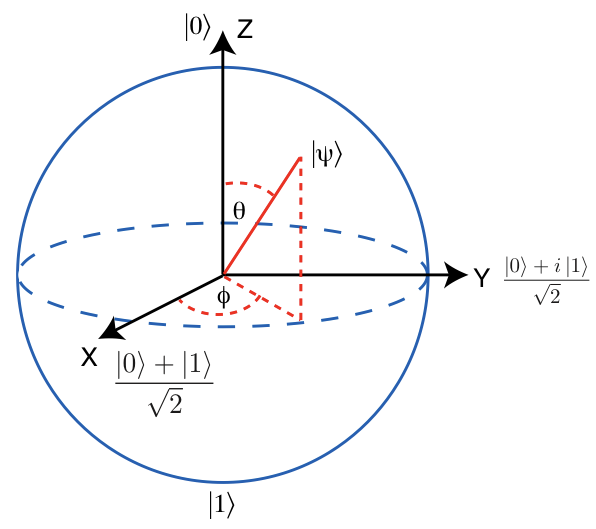
\includegraphics[width=0.60\textwidth]{figures/Bloch_sphere.png}
\caption{Representation of the qubit in the state $\vert \psi \rangle$ in the
Bloch sphere.}
\label{fig:bloch}
\end{figure}

The qubit's 0 and 1 states are mathematically represented as follows:

\begin{linenomath}
\begin{equation}
	\vert 0 \rangle = \begin{pmatrix} 1 \\ 0 \end{pmatrix}, \vert 1 \rangle = \begin{pmatrix} 0 \\ 1 \end{pmatrix}
\label{eq:qu01}
\end{equation}
\end{linenomath}

As a consequence of this mathematical description, unlike a bit, a qubit is not 
limited to being in one of these two states. Qubits can exist in what's known as
a superposition of states. A superposition is a linear combination of two basis 
vectors. Mathematically:

\begin{linenomath}
\begin{equation}
	\vert \psi \rangle = \alpha \vert 0 \rangle + \beta \vert 1 \rangle = \alpha \begin{pmatrix} 1 \\ 0 \end{pmatrix} + \beta \begin{pmatrix} 0 \\ 1 \end{pmatrix} = \begin{pmatrix} \alpha \\ \beta \end{pmatrix}
\label{eq:supos}
\end{equation}
\end{linenomath}
where $\alpha$ and $\beta$ are complex numbers that satisfy:
\begin{linenomath}
\begin{equation}
	\alpha\alpha^* + \beta\beta^* =1
\label{eq:norm}
\end{equation}
\end{linenomath}

\subsection{Quantum Circuits}
\label{sec:circuit}

Quantum circuits are a common means of visually representing the sequence of 
operations that are performed on qubits during a quantum computation. They 
consist of a set of operations (gates) applied to a set of qubits (wires). Each 
wire in the diagram represents a qubit. Circuits are read from left to right, 
and this is the order in which operations are applied.
An example of a quantum circuit is shown in Figure~\ref{fig:circuit}.

\begin{figure}[!htbp]
\centering
	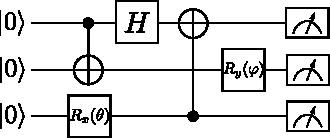
\includegraphics[width=0.60\textwidth]{figures/qcircuit.pdf}
\caption{Example of a quantum circuit. This circuit has three qubits that start 
in the state $\vert 0 \rangle$, performs five operations, and measures every 
qubit at the end of the circuit.}
\label{fig:circuit}
\end{figure}

A quantum computation is all about manipulating qubit states by using gates and
seeing the outcome of such manipulations by measuring the qubits.

\subsection{Flipping qubits}
\label{sec:flip}

Performing quantum operations involves multiplication by matrices that send 
valid, normalized quantum states to other normalized quantum states. The 
simplest quantum operation as the following effect:

\begin{linenomath}
\begin{equation}
	X\vert 0 \rangle = \vert 1 \rangle, \
	X\vert 1 \rangle = \vert 0 \rangle
\label{eq:flip}
\end{equation}
\end{linenomath}

Known as bit flip, $Pauli\rm{-}X$ or $NOT$ gate, it can be mathematically represented as:

\begin{linenomath}
\begin{equation}
	X = \begin{pmatrix}
	0 & 1 \\
	1 & 0
	\end{pmatrix}
\label{eq:flipX}
\end{equation}
\end{linenomath}

Figure~\ref{fig:circuitX} represents the qubit flip gate in a quantum circuit 
diagram.

\begin{figure}[!htbp]
\centering
	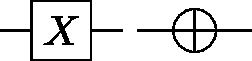
\includegraphics[width=0.40\textwidth]{figures/X.pdf}
\caption{The $Pauli\rm{-}X$ or $NOT$ gate in a quantum circuit.}
\label{fig:circuitX}
\end{figure}

Equation~\ref{eq:flipped} shows the mathematical operation of applying the $NOT$
gate to a qubit in state $\vert 0 \rangle$ flipping it to state $\vert 1 \rangle$.

\begin{linenomath}
\begin{equation}
	X\vert 0 \rangle=\begin{bmatrix} 0 & 1 \\ 1 & 0 \end{bmatrix} \begin{bmatrix} 1 \\ 0 \end{bmatrix} = \begin{bmatrix} 0 \\ 1 \end{bmatrix} = \vert 1 \rangle
\label{eq:flipped}
\end{equation}
\end{linenomath}

\subsection{Rotations, rotations, rotations: the $R_X(\theta)$, $R_Y(\theta)$, and $R_Z(\theta)$ Gates}
\label{sec:rot}

One of the most relevant operations to the qubit in the context \gls{qml} are 
the $R_X(\theta)$, $R_Y(\theta)$, and $R_Z(\theta)$ gates because they can be 
used to rotate the qubit state in the Bloch sphere. This means qubits can be 
manipulated as a function of a parameter, an angle, in order to find an optimum 
in the quantum algorithm being designed. This concept is analogous to using 
weights in Neural Networks. In the same manner, the value of the angles used in 
the rotations are the parameter upon which the \gls{qml} algorithm is going to 
be trained.

As it was shown, a qubit can be represented in 3D-space by the Bloch sphere. 
Using the same representation, $R_X(\theta)$, $R_Y(\theta)$, and $R_Z(\theta)$ 
are shown in Figure~\ref{fig:rots}.

\begin{figure}[!htbp]
\centering
	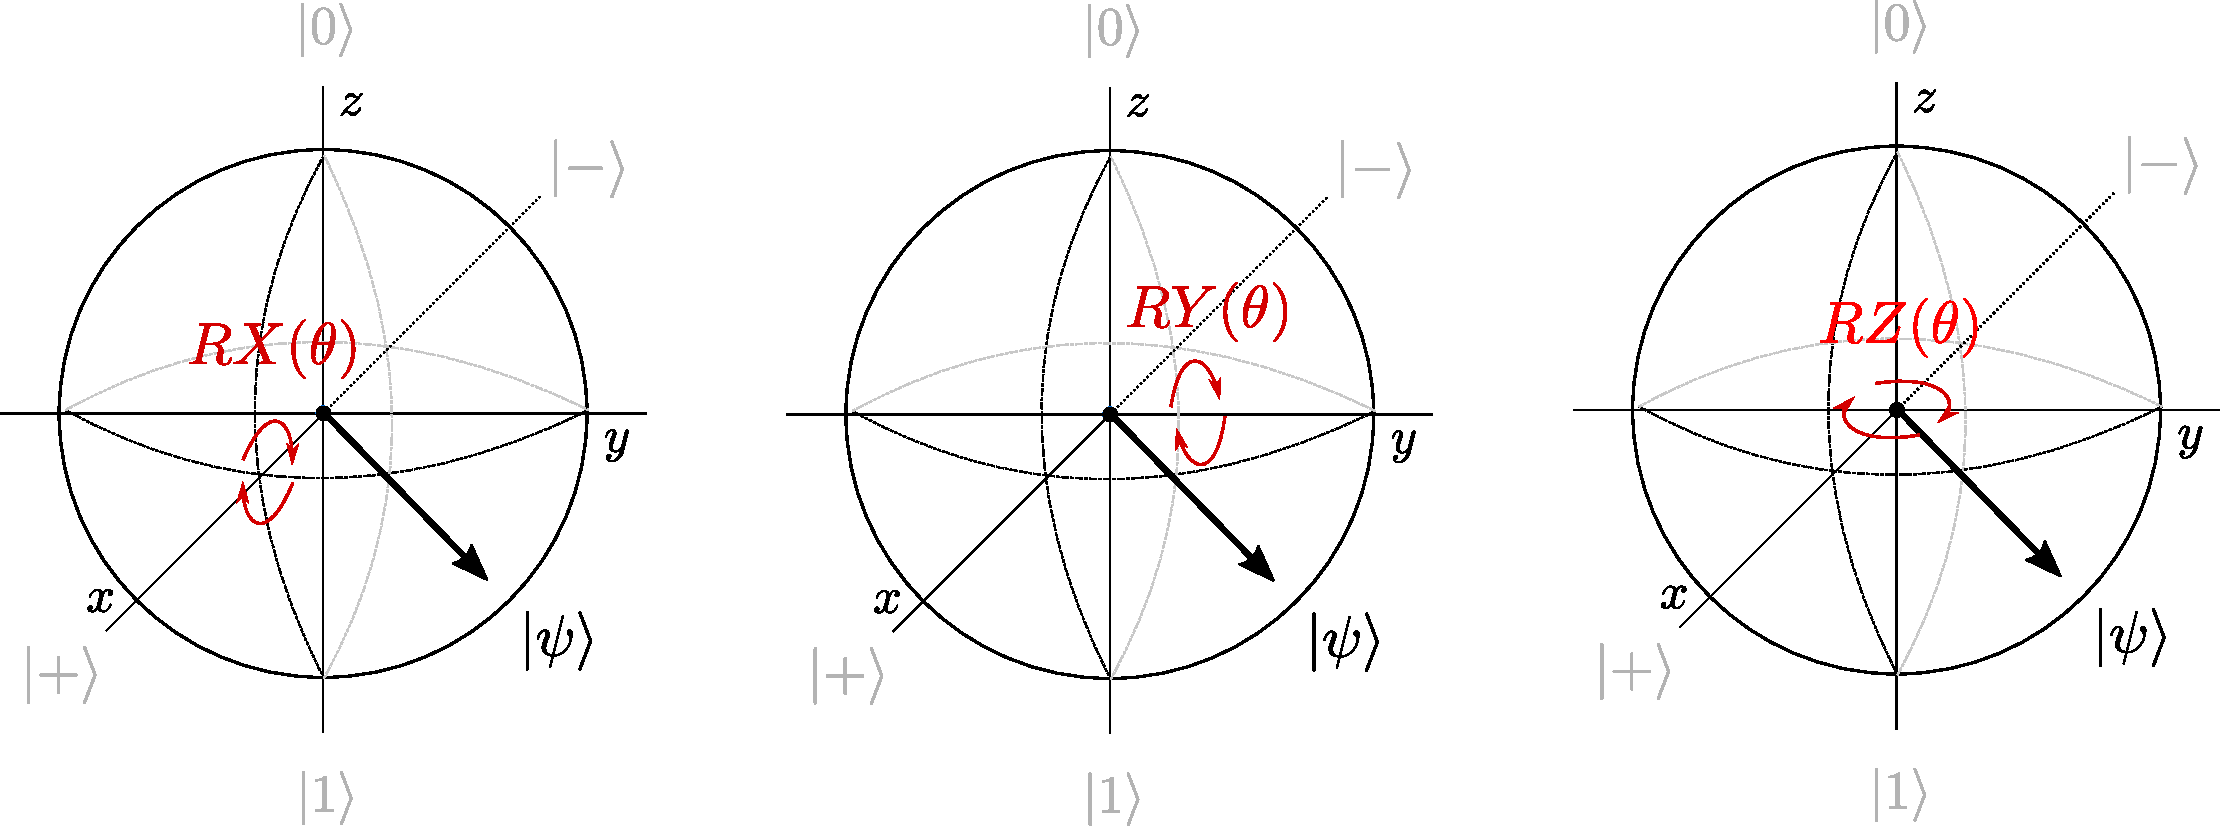
\includegraphics[width=1\textwidth]{figures/rotations.pdf}
\caption{The $R_X(\theta)$, $R_Y(\theta)$, and $R_Z(\theta)$ gates in a the Bloch sphere.}
\label{fig:rots}
\end{figure}

The matrix representation of these rotations:

\begin{linenomath}
\begin{equation}
	R_X(\theta)=\begin{pmatrix}
\cos(\frac{\theta}{2}) & -i\sin(\frac{\theta}{2}) \\
-i\sin(\frac{\theta}{2}) & \cos(\frac{\theta}{2})
\end{pmatrix} 
\label{eq:rotx}
\end{equation}
\end{linenomath}
\begin{linenomath}
\begin{equation}
	R_Y(\theta)=\begin{pmatrix}
\cos(\frac{\theta}{2}) & -\sin(\frac{\theta}{2}) \\
\sin(\frac{\theta}{2}) & \cos(\frac{\theta}{2})
\end{pmatrix}
\label{eq:roty}
\end{equation}
\end{linenomath}
\begin{linenomath}
\begin{equation}
	R_Z(\theta)=\begin{pmatrix}
e^{\frac{-i\theta}{2}} & 0 \\
0 & e^{\frac{i\theta}{2}}
\end{pmatrix}
\label{eq:rotz}
\end{equation}
\end{linenomath}

Figure~\ref{fig:rotscirc} represents the $R_X(\theta)$, $R_Y(\theta)$, 
and $R_Z(\theta)$ gates in a quantum circuit diagram.

\begin{figure}[!htbp]
\centering
	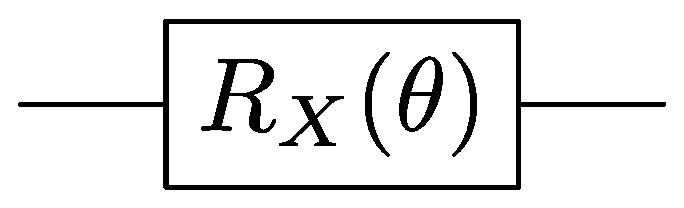
\includegraphics[width=0.30\textwidth]{figures/RX.pdf}
	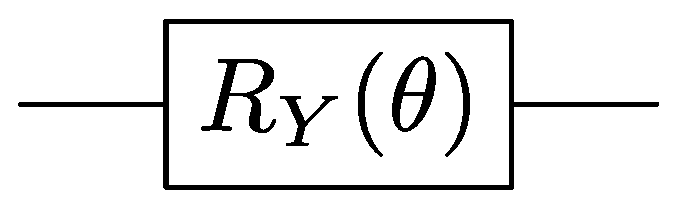
\includegraphics[width=0.30\textwidth]{figures/RY.pdf}
	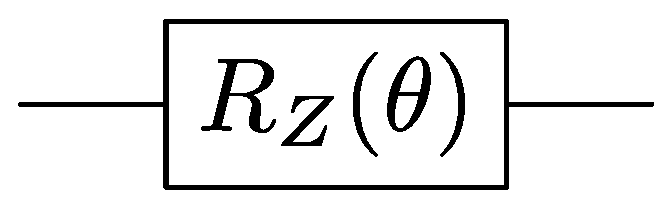
\includegraphics[width=0.30\textwidth]{figures/RZ.pdf}
\caption{The $R_X(\theta)$, $R_Y(\theta)$, and $R_Z(\theta)$ gates in a quantum 
circuit diagram.}
\label{fig:rotscirc}
\end{figure}

\subsection{Superposition and the $Hadamard$ Gate}
\label{sec:hada}

The Hadamard gate, $H$, is a fundamental quantum gate that allows to move away 
from the poles of the Bloch sphere, and create a superposition of $\vert 0 \rangle$ 
and $\vert 1 \rangle$ as follows:

\begin{linenomath}
\begin{equation}
H \vert 0 \rangle = \frac{1}{\sqrt{2}}(\vert 0 \rangle + \vert 1 \rangle)
\label{eq:hadamap}
\end{equation}
\end{linenomath}

It is mathematically represented as:

\begin{linenomath}
\begin{equation}
H = \frac{1}{\sqrt{2}} \begin{pmatrix}
1 & 1 \\
1 & -1
\end{pmatrix}
\label{eq:hada}
\end{equation}
\end{linenomath}

Figure~\ref{fig:hada} represents the $Hadamard$ gate in a quantum circuit diagram.

\begin{figure}[!htbp]
\centering
	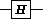
\includegraphics[width=0.20\textwidth]{figures/H.pdf}
\caption{The $H$ gate in a quantum circuit diagram.}
\label{fig:hada}
\end{figure}

Equation~\ref{eq:hadaop} shows the mathematical operation of applying the $H$
gate to a qubit in state $\vert 0 \rangle$ mapping it to a state in a superposition,
commonly written as $\vert + \rangle$.

\begin{linenomath}
\begin{equation}
H\vert 0 \rangle=\frac{1}{\sqrt{2}}\begin{bmatrix} 1 & 1 \\ 1 & -1 \end{bmatrix} \begin{bmatrix} 1 \\ 0 \end{bmatrix} = \frac{1}{\sqrt{2}}\begin{bmatrix} 1 \\ 1 \end{bmatrix} = \frac{1}{\sqrt{2}} (\vert 0 \rangle + \vert 1 \rangle) = \vert + \rangle
\label{eq:hadaop}
\end{equation}
\end{linenomath}

\subsection{Multiple Qubit States}
\label{sec:multq}

To describe a state of 2 qubits, 4 complex amplitudes are required:

\begin{linenomath}
\begin{equation}
\vert \psi \rangle = \psi_{00}\vert 00 \rangle + \psi_{01}\vert 01 \rangle + \psi_{10}\vert 10 \rangle + \psi_{11}\vert 11 \rangle = \begin{bmatrix} \psi_{00} \\ \psi_{01} \\ \psi_{10} \\ \psi_{11} \end{bmatrix}
\label{eq:multiq}
\end{equation}
\end{linenomath}

Such that the normalization condition is respected:

\begin{linenomath}
\begin{equation}
	|\psi_{00}|^2 + |\psi_{01}|^2 + |\psi_{10}|^2 + |\psi_{11}|^2 = 1
\label{eq:multinorm}
\end{equation}
\end{linenomath}

Qubits $\vert a \rangle$ and $\vert b \rangle$ are two separate qubits such that:

\begin{linenomath}
\begin{equation}
	\vert a \rangle = \begin{bmatrix} a_0 \\ a_1 \end{bmatrix}, \vert b \rangle = \begin{bmatrix} b_0 \\ b_1 \end{bmatrix}
\label{eq:ab}
\end{equation}
\end{linenomath}

The kronecker product is used to describe the collective state. The collective 
state of qubits $\vert a \rangle$ and $\vert b \rangle$ is described as follows:

\begin{linenomath}
\begin{equation}
\vert ba \rangle = \vert b \rangle \otimes \vert a \rangle = \begin{bmatrix}
b_0 \times \begin{bmatrix} a_0 \\ a_1 \end{bmatrix} \\
b_1 \times \begin{bmatrix} a_0 \\ a_1 \end{bmatrix}
\end{bmatrix} = \begin{bmatrix} b_0 a_0 \\ b_0 a_1 \\ b_1 a_0 \\ b_1 a_1 \end{bmatrix} 
\label{eq:kron1}
\end{equation}
\end{linenomath}
\begin{linenomath}
\begin{equation}
\vert ba \rangle = b_0a_0\vert 00 \rangle + b_0a_1\vert 01 \rangle + b_1a_0\vert 10 \rangle + b_1a_1\vert 11 \rangle
\label{eq:kron2}
\end{equation}
\end{linenomath}

For a computation with $n$ qubits, a computer needs to keep track of $2^n$
complex amplitudes. This is the reason why quantum computers are difficult to 
simulate. A modern laptop can simulate a general quantum state of around 10 
qubits, but simulating 100 qubits is too difficult even for the largest 
supercomputers.

\subsection{Entanglement and the $CNOT$ Gate}
\label{sec:cnot}

Until now, only gates that act on a single qubit have been described. In order
to complete all the "ingredients" necessary, gates that act on multiple qubits
are needed in order to entangle multiple qubits.

When 2 qubits are entangled, by knowing the state of one qubit, the state of 
other becomes known as well. The $CNOT$ operation changes the state of a target
qubit depending on the state of a control qubit. When these two concepts are 
merged, qubits can be entangled in quantum computers.

By definition, a state is entangled if it cannot be described as a tensor product
of individual qubit states. An entangled state can only be described by specifying 
the full state. One example of an entangled state:

\begin{linenomath}
\begin{equation}
	\vert ba \rangle = \frac{1}{\sqrt{2}} (\vert 00 \rangle + \vert 11 \rangle)
\label{eq:entg}
\end{equation}
\end{linenomath}

In order to describe this state using the kronecker tensor one needs to find 
$a_0$, $a_1$, $b_0$ and $b_0$ such that: 

\begin{linenomath}
\begin{equation}
b_0a_0=1,
b_0a_1=0, 
b_1a_0=0,
b_1a_1=1
\label{eq:entgcond}
\end{equation}
\end{linenomath}

Each variable appears in two equations, one of which is equal to 1, and the other
to 0. But for any of the 0 ones to be true, at least one variable needs to be 0,
and that would immediately contradict the other equation. Therefore, there is no
solution, it's not possible to describe this state as two separate qubits. They 
are entangled.

The $controlled\rm{-}NOT$ or $CNOT$ gate can make an entangled state by performing 
the $Pauli\rm{-}X$ operation on one target qubit depending on the state of 
another control qubit. Mathematically represented as:

\begin{linenomath}
\begin{equation}
CNOT = \begin{pmatrix}
1 & 0 & 0 & 0 \\
0 & 0 & 0 & 1 \\
0 & 0 & 1 & 0 \\
0 & 1 & 0 & 0 
\end{pmatrix}
\label{eq:cnot}
\end{equation}
\end{linenomath}

Figure~\ref{fig:cnot} represents the $CNOT$ gate in a quantum circuit diagram.

\begin{figure}[!htbp]
\centering
	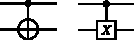
\includegraphics[width=0.40\textwidth]{figures/CNOT.pdf}
\caption{The $controlled\rm{-}NOT$ or $CNOT$ gate in a quantum circuit.}
\label{fig:cnot}
\end{figure}

Qubits $\vert q_0 \rangle$ and $\vert q_1 \rangle$ are two separate qubits such 
that:

\begin{linenomath}
\begin{equation}
\vert q_0 \rangle = \frac{1}{\sqrt{2}} (\vert 0 \rangle + \vert 1 \rangle)
\label{eq:q0}
\end{equation}
\end{linenomath}

\begin{linenomath}
\begin{equation}
\vert q_1 \rangle = \vert 0 \rangle
\label{eq:q1}
\end{equation}
\end{linenomath}

The collective state is defined as $\vert q_0q_1 \rangle = \frac{1}{\sqrt{2}} 
(\vert 00 \rangle + \vert 01 \rangle)$ which is not entangled. Now, if the gate
$CNOT$ is applied to the collective state as in Equation~\ref{eq:cnot1}, an
entangled state is achieved.

\begin{linenomath}
\begin{equation}
CNOT\vert q_0q_1 \rangle = \frac{1}{\sqrt{2}} \begin{bmatrix} 1 & 0 & 0 & 0 \\ 0 & 0 & 0 & 1 \\ 0 & 0 & 1 & 0 \\ 0 & 1 & 0 & 0 \end{bmatrix} \begin{bmatrix} 1\\1\\0\\0 \end{bmatrix} = \frac{1}{\sqrt{2}} \begin{bmatrix} 1\\0\\0\\1 \end{bmatrix} 
\label{eq:cnot1}
\end{equation}
\end{linenomath}

\begin{linenomath}
\begin{equation}
CNOT\vert q_0q_1 \rangle = \frac{1}{\sqrt{2}} (\vert 00 \rangle + \vert 11 \rangle)
\label{eq:cnot2}
\end{equation}
\end{linenomath}

\subsection{qGANS}
\label{sec:qgan}

QGANs are fundamentally composed of two Quantum Neural Networks (QNNs) - a generator and a discriminator one - that compete between each other. The generative network generates candidates while the discriminative network evaluates them. The contest operates in terms of data distributions. Typically, the generative network learns to map from a latent space to a data distribution of interest, while the discriminative network distinguishes candidates produced by the generator from the true data distribution. The generative network's training objective is to increase the error rate of the discriminative network (i.e., "fool" the discriminator network by producing novel candidates that the discriminator thinks are not synthesized (are part of the true data distribution)).
